%!TEX root = ../../main.tex

\chapter{Application structure}
% TODO: Describe a generic application and how it should be structured. For instance the use of the topbar or sidemenu. Also talk about contextual menus.

\section{Top Bar}
\index{Action bar}
\index{Top bar}
All activities in every application, except the home-activity in the Launcher-application,  must have a top bar. This top bar should look like the example in \figref{fig:top_bar_example}. This top bar should provide a short and simple title with enough information to allow the user to know where in the application he or she is. The height of the top bar must be $56dp$. Furthermore, this top bar must include at the two buttons described in \secref{sec:back_button} and \secref{sec:help_button}.

\begin{figure}[!htbp]
        \centering
        
\includegraphics[width=0.75\textwidth]{pictures/application_structure/topbar}
        \caption{Top bar example}
        \label{fig:top_bar_example}
\end{figure}

\begin{note}
    Such a top bar is easily achieved by letting all of your \androidinline{Activity} extend the \androidinline{GirafActivity} from the \gc library. Doing this will also implement the back button described in \secref{sec:back_button}.
\end{note}

\subsection{Back Button}
\label{sec:back_button}
The left-most button in the top bar must be a back button. This button must have exactly the same functionality as the back button on all Android devices. The icon of this button must be... \todo{Insert reference to the section where icons are described}...

\subsection{Help Button}
\label{sec:help_button}
The right-most button in the top bar must be a help button. This button must provide the user with some useful help information regarding the current screen which the user is presented with. For instance if the user is assigning applications to users, the help might be a guide on how to do this correctly.

\FloatBarrier


\section{Side Bar}
\index{Side bar}

Side bars need not, but may be contextual. It is recommended to use side bars to switch between content of applications. A side bar should look like \figref{fig:side_bar_example}.

\begin{figure}[!htbp]
        \centering
        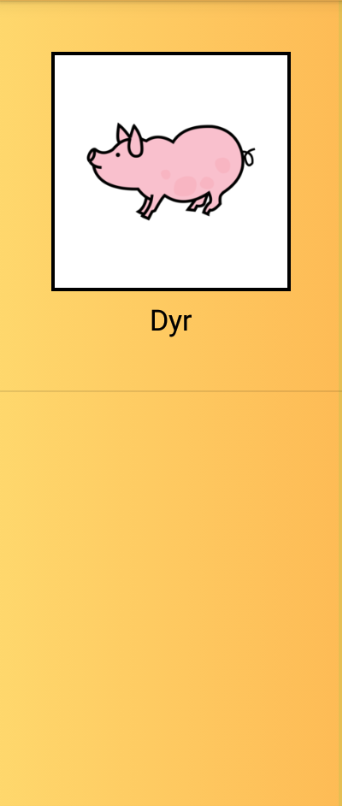
\includegraphics[width=0.25\textwidth]{pictures/application_structure/sidebar}
        \caption{Side bar example}
        \label{fig:side_bar_example}
\end{figure}

\FloatBarrier


\section{Bottom bar}
\index{Bottom bar}
Bottom bars should be entirely contextual and depend on the current content displayed in the current \androidinline{Activity}. A bottom bar should look like \figref{fig:bottom_bar_example}.

\begin{figure}[!htbp]
        \centering
        
\includegraphics[width=0.75\textwidth]{pictures/application_structure/bottombar}
        \caption{Bottom bar example}
        \label{fig:bottom_bar_example}
\end{figure}

\FloatBarrier


\section{Content}
The main content of applications should be in the center of the layout and any menu bars should be above, under, and to the sides of the main content. 

\begin{note}
We recommend using Android \androidinline{Fragment} instances to manage content of an \androidinline{Activity} if the main content of an Android \androidinline{Activity} needs to change between different content that needs to be controlled differently. 
\end{note}


\section{Clickable Elements}
All elements that are clickable must have a safety-distance to other elements. This will ensure that the user does not accidentally press the wrong thing and ultimately does something wrong. This safety distance may be achieved using several different methods. Please refer to the following sections. \figref{fig:correct_element_spacing} shows an example of correct item spacing while \figref{fig:incorrect_element_spacing} shows an example of incorrect item spacing.
\\\\
Elements must have a safety distance to \ldots
\index{Margin}
\begin{itemize}
        \item Other clickable elements
        \item Borders of it's container
        \item Borders of the tablet
\end{itemize}

\begin{figure}[!htbp]
    \centering
    \begin{subfigure}[t]{0.4\textwidth}
        \centering
        
\includegraphics[scale=0.1]{correct_element_spacing}
        \caption{Correct item spacing}
        \label{fig:correct_element_spacing}
    \end{subfigure}
    \hspace{5em} 
    \begin{subfigure}[t]{0.4\textwidth}
        \centering
        
\includegraphics[scale=0.1]{incorrect_element_spacing}
        \caption{Incorrect item spacing}
        \label{fig:incorrect_element_spacing}
    \end{subfigure}
    
    \caption{Examples of correct and incorrect element spacing}
    \label{fig:element_spacing_examples}
\end{figure}

\subsection{Element Margin}
\index{Margin}
Elements may be spaced apart from each other using margin on the individual elements. The distance between the elements should be consistent throughout all activities of any given application. \figref{fig:element_margin_example} shows an example of the margin for a given element.. 

\begin{figure}[h]
        \centering
        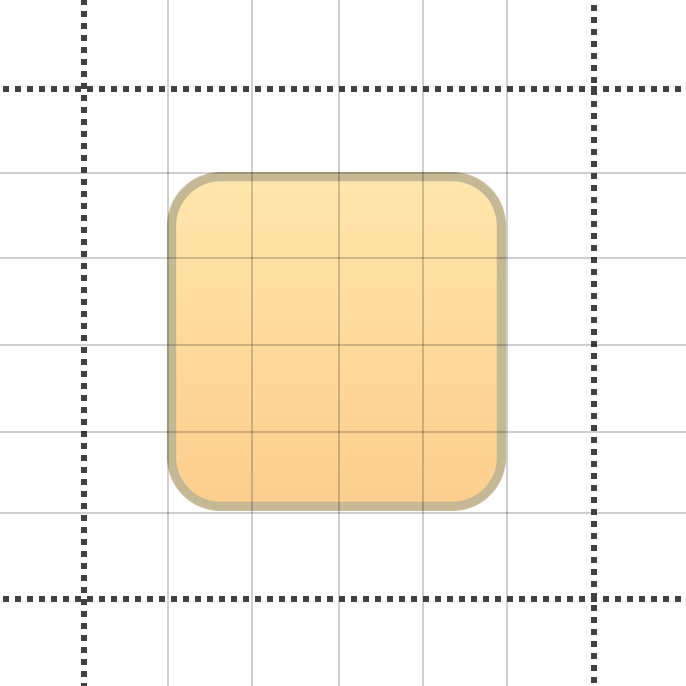
\includegraphics[width=0.25\textwidth]{element_margin_example}
        \caption{Example of element margin}
        \label{fig:element_margin_example}
\end{figure}

\begin{note}
        If margin is used inside a container each element with margin will also be a certain distance from the borders of that specific container. If, for instance, an element has a margin of $10$, then this element would be a distance of $10$ from the borders of the container. This means that there \textit{might} not be need for any padding on the given container.
\end{note}

\subsubsection{Consistent Margin}
\index{Margin}
Elements of the same type appearing in the same context must have the same distance to other elements. However, if the elements appear in an order, for example a horizontal list, the first and last element may differ. For instance, the first element may have a smaller left-margin and the last element may have a smaller right-margin. \figref{fig:element_margin_consistency} shows an illustration of this example.

\begin{figure}[h]
        \centering
        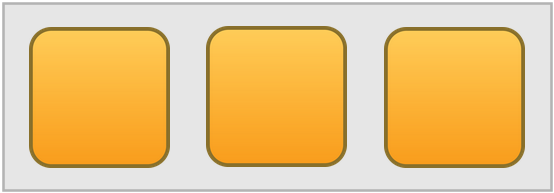
\includegraphics[width=0.45\textwidth]{element_margin_consistency}
        \caption{Example of element margin}
        \label{fig:element_margin_consistency}
\end{figure}


\subsection{Container Padding}
\index{Padding}
Each container should provide some padding for its content. This padding should be somewhat identical to the spacing between elements inside the container. \figref{fig:container_padding_example} shows an example of a container with padding. 

\begin{figure}[h]
        \centering
        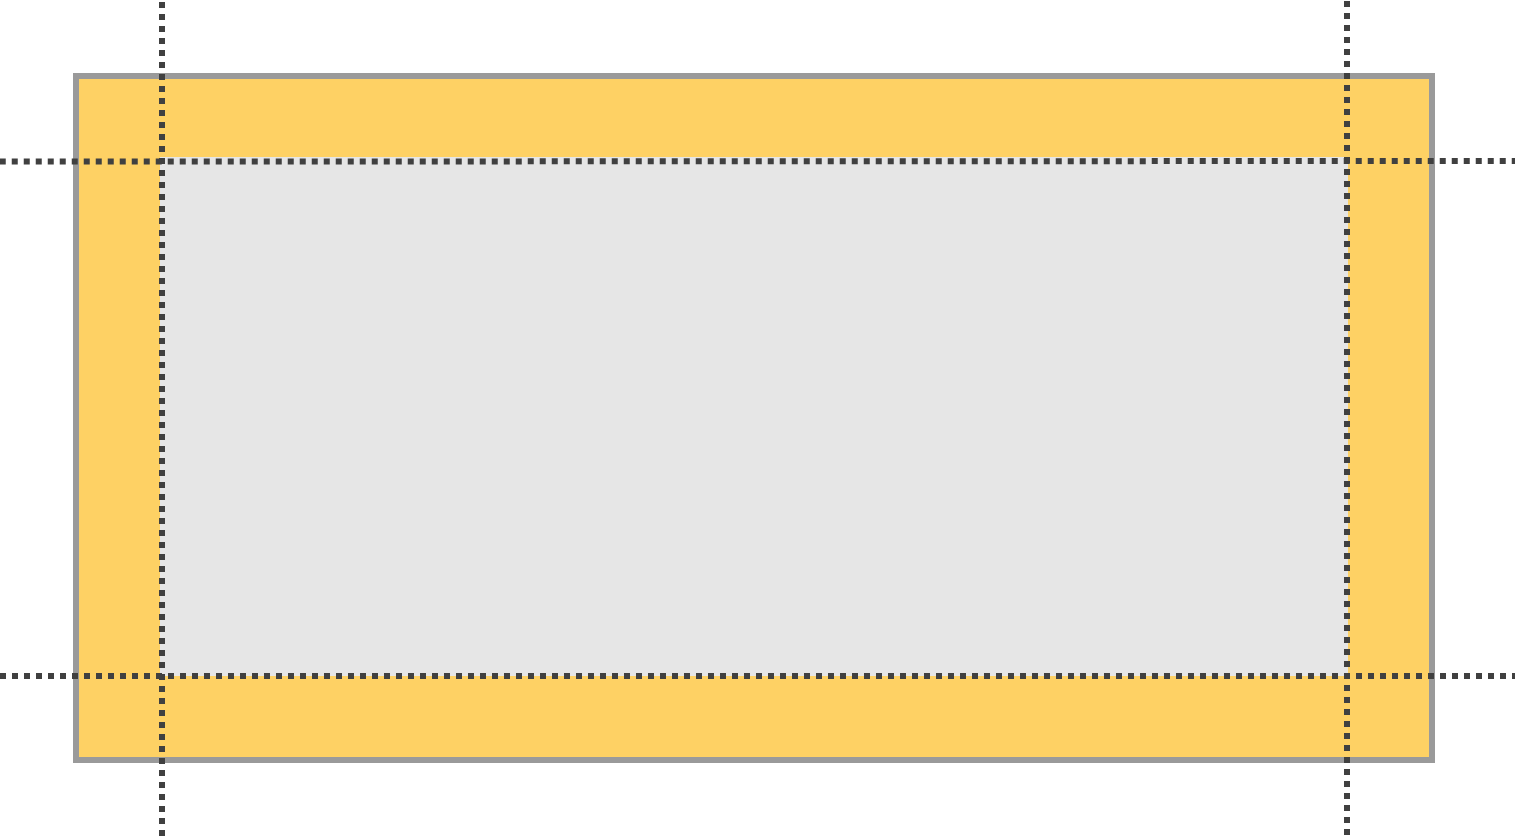
\includegraphics[width=0.65\textwidth]{container_padding_example}
        \caption{Example of a container with padding}
        \label{fig:container_padding_example}
\end{figure}

\begin{note}
        Whenever the content of the container can be scrolled through (for example a \texttt{GridView}) a property called \texttt{clipToPadding} must be set to \texttt{false}. Please refer to the \href{http://developer.android.com/reference/android/view/ViewGroup.html#attr_android:clipToPadding}{Android documentation} for additional information.
\end{note}\todo{The effect of this could be explained more clearly using a figure}
